% File 'gusample.tex' -- Mark Maloof, Michael A. Covington, Isidor Ruderfer
% (Revised 15 December 2010)
% This is an example of how to format a thesis or dissertation using LaTeX 2e
% with 'guthesis.sty' VERSION 3.4 OR LATER.

\documentclass[12pt]{report}

\usepackage{url}
\usepackage[numbers,sort]{natbib}
\usepackage{graphicx}
\usepackage{amsmath}
\usepackage{amssymb}
\usepackage{algorithm}
\usepackage{algorithmic}

% If there are any other \usepackage commands, put them here.

\usepackage{lib/style/guthesis} % Must be the last package

\newtheorem{theorem}{Theorem}[section]
\newenvironment{proof}[0]{\textit{Proof.}}{}
\newcommand{\qed}{\hfill $\Box$}

% To comment out multiple lines of text.
\long\def\comment#1{}

\title{Peering Through Censorship:\\Tackling Internet Censorship Using P2P Networking}

\author{Eliana V. Troper}

\previousdegree{A.B.}

\thisdegree{Master of Science}  % or Doctor of Philosophy, etc.

\thisdiscipline{Computer Science}

\thesistype{Thesis}     % or Dissertation

% defense or approval date, not today's date...
\thesisday{11}
\thesismonth{April}
\thesisyear{2023}

\professor{Micah Sherr}
%\secondprofessor{Alonzo Church}   % Only if you have 2 major professors!

\fulltitle{Peering Through Censorship: Tackling Internet Censorship Using P2P Networking}

% TODO: Update this
\indexwords{Word~processing, Computer~typesetting, Computer~graphics,
            Style~sheets, Typography, Dissertations, Theses~(academic)}

\dean{Alexander Sens}

\memberi{Lisa Singh}
\memberii{Benjamin Ujcich}
% Use \memberiii, \memberiv, \memberv for up to 3 more members if needed.

\begin{document}

\pagenumbering{roman}

\maketitle    % Creates title page, copyright page if any, and approval page.

\begin{abstract}
TODO: Optional for master's thesis but these are nice (max 350 words)
\end{abstract}


\chapter*{Dedication}

TODO: Optional

\pseudochapter{Acknowledgments}

TODO

\tableofcontents

\listoffigures  % Optional - Omit this line if you don't want a list of figures.
\listoftables   % Optional - Omit this line if you don't want a list of tables.

\newpage

\pagenumbering{arabic}  % Ordinary pages have Arabic numerals.

\chapter{Introduction}

People us the internet to communicate and share a variety of content. Some entities choose to censor internet connections. These entities may range from individual network administrators to a full nation-state. In this paper, we explore the background and current state of censorship circumvention, and then design and build a system which tackles several of the limitations present in state of the art systems. [LATER: Add xrefs to sections]

We begin by exploring what we mean by censorship circumvention and establishing baseline terminology for this subdiscipline. We then explore the present theory behind approaches to censorship circumvention. We address the ethics of censorship circumvention as a field, and how the field originated and how that affects the current state of the field.

We then propose several ways to classify existing systems to allow for some comparison between them, and we then explore existing and past systems to understand where the field stands, and where limitations occur. We emphasize systems that are either cutting edge or in active use in the real world.

We also provide an overview of the state of peer to peer (P2P) networking, focusing on succesful project operating in the real world. We provide a deeper dive into the Interplanetary File System (IPFS) and the underlying networking library, LibP2P. These programs are used extensively in out proposed system.

Having outlined what is and has succeeded in censorship circumvention in both the real world and theory, we propose a system that addresses the flaws of the current cutting edge systems. We call this system CN. [TODO: fn code name] We discuss the architecture of this system, putting a particular emphasis on the underlying data structure and network topology.

We build this system and build a benchmarking tool and other apps on top of this system. We use this benchmarking tool to show that the system functions with strong performance. We then begin to simulate a censor based upon theoretical and real world adversaries, and then benchmark the system again, showing that even under severely censored circumstances, we are able to maintain [adequate/good/strong] performance. We also explore what regions of the world would have to operate in more censored circumstances at present.

We then conclude and offer some opportunities for future work.

\chapter{Background}

TODO

\section{What is censorship circumvention?}

When we discuss the subfield of censorship circumvention when discussing networking and security, we are \emph{not} discussing all forms of censorship that a web user might face - we are discussing censorship on-the-wire of active internet traffic, which usually consists of blocking access to specific services. We do not consider a service blocking certain conduct (e.g. a social network restricting hate speech) the censorship that we are circumventing. We aim to allow a use to connect to any service they would like (notwithstanding technical limitations) - not to allow a user to use any service how they would like. Throughout this paper, when we mention censorship, we mean on-the-wire censorship of reaching services.

\subsection{Ethics}

We recognize that some users run heinous services on the web - most of which are illegal in any existing jurisdiction. We believe that the best approach for ceasing access to these heinous services is best done through a legal system - ie, investigating and identifying the perpetrator(s), turning off the service directly, and prosecuting any perpetrator(s) of said acts. We note that most morally reprehensible acts that are frequently associated with anonymity and censorship circumvention systems involve actions that occur in the real world (e.g. exploitation of children, weapon/drug/human trafficking all involve actions that occur in the real world either prior to distribution on the internet or triggered by actions on the internet).

The only notable class of crime which can occur without physical, real-world actions is piracy/IP violations. We believe that targetted legal actions (e.g. DMCA takedowns) can mitigate the issue, and that the cost of further mitigation through censorship would lead to large collateral damage of legal content and a chilling effect of legal speech and usage of the web, and as such the possibility of a circumvention system being used for piracy/IP violations is an acceptable risk given the ability to mitigate damage through the legal system.

\subsection{Threat model and adversary}

Censorship circumvention is an abstract concept, and approaching it in a scientific way requires properly defining and scoping the task. We have already defined the task, [TODO: xref] and must now scope the problem. We will scope our problem by creating a \textbf{threat model} of the censor we are aiming to thwart, termed \textbf{the adversary}.

An adversary has an \textbf{area of influence}. This is an area an adversary controls the network of, and can control (either directly or through compulsion) any service providers within. We assume an adversary may have an area of influcence consisting of several nations, with at least one nation outside of the area of influence of \emph{any} censor.\footnote{This does not mean that this nation does not have the technical capability to censor, but rather does not perform any censorship either directly or via threatening a start of censorship.}

Our adversary has effectively infinite resources, but is bound by the laws of physics and as such is bounded by the difficulty of computational problems (and the known solutions to these problems, e.g. even if P=NP, the solution is not known, and as such cannot be used). These resources may include labor, capital, technical expertise, and total control of the legal system.

We also assume that our adversary has access to the source code of any circumvention system available, and knowledge of the existence of our circumvention system. We discuss why security through obscurity cannot be used in an effective circumvention system in [TODO: xref].

We also assume that our adversary only takes actions \textbf{on-the-wire} and at \textbf{service providers} within their area of influence - effectively, the adversary isn't interested in any individual in particular and is performing a dragnet operation, rather than an operation targetting a specific entity. We can use a thought experiment to justify this: if an adversary had a person looking over your shoulder or using video surveillance, they could simply look at what you are doing and punish you directly, no need to expend the resources needed to censor the web.

We assume our adversary has some interest in the utility of the internet and certain technologies on the internet. This means two things: an adversary will not shut down the internet in it's entirety\footnote{Internet shutdowns are a trivial way to censor forbidden internet usage - at the expense of shutting down any non-forbidden usage. [TODO: Discuss prior shut downs in another section and xref]} and an adversary has some threshold of unacceptable collateral damage caused by potential censorship techniques.\footnote{Similar to a full internet shutdown, if an adversary wanted to block all access to a specific HTTP site, they could block \emph{all} HTTP traffic, at the expense of blocking every HTTP site. This piecemeal web censorship could even be thwarted with a circumvention system that simply proxies HTTP traffic outside of the area of influence within an unblocked protocol and connects to HTTP sites from outside the area of influcence. This starts to show that any non-complete shutdown of internet traffic may have gaps for circumvention techniques. We discuss collateral damage further in [TODO: xref].}

Finally, we note that any technique that subverts this adversary will also work when weakening the strength of these assumptions - e.g. if the adversary controls one nation instead of several, we have more area to run a circumvention system from; if the adversary is only willing to take actions at service providers and not on-the-wire, anything that can thwart an adversary that takes both actions could trivially thwart the adversary that only performs actions at one. We also note that a system could detect the type of actions an adversary is taking and maximize performance based upon what subset of possible actions an adversary is taking - e.g. an adversary that is not touching services leaves an easy path for a circumvention system to use - those services themself.

\subsection{Current theory of censorship circumvention}

TODO

[TODO: Mention parrot is dead]

\subsection{Origination of censorship circumvention}

TODO

\section{Prior techniques}

TODO

[TODO: Do mention some things like shadowsocks that are in use but are even further from academics]

\subsection{[Point to point obfuscation]}

TODO

\subsubsection{OBFS and Scramblesuit}

TODO

\subsection{[P2P and P2P-like]}

TODO

\subsubsection{Snowflake}

TODO

[TODO: Iran case study]

\subsubsection{MassBrowser}

TODO

\subsection{High-reliability channels}

TODO

\subsubsection{Domain fronting}

TODO

\subsubsection{Raven}

TODO

\subsection{Decoy routing}

TODO

\section{Real world observations}

TODO

\subsection{Real world vs. academic theory}

TODO

\section{P2P networking}

TODO

\subsection{IPFS}

TODO

\chapter{System design}

We saw that several circumvention systems work given the constraints they were designed for, however, these constraints are either too loose and have known real-world failures under our adversary model, the systems are too difficult to deploy, or they have hit scalability issues.

We propose a system with a clear theoretical backing and acheivable goals based on both theory and real-world observations.

\section{Theory and goals}

First, we want to define system goal and highlight some non-goals that are close to censorship circumvention, but are not directly used for them.

We aim to thwart the adversary we outline in [xref]. We will rely heavily on the concept of collateral damage. [TODO: Discuss collateral damage further]

We are \emph{not} aiming to provide anonymity.\footnote{Perhaps our system could be used to access an anonymity system, but we do not want to guarentee anonymity or guarentee that the system will not leak information that may break anonymity, though we are not delibrately trying to break anonymity, we are also not evaluating our system for it at this point.} We feel the need to emphasize this, as most current systems that are functional in the real world are used as pluggable transports by Tor.\footnote{Our system could be used as a PT, as we do have a golang implementation.} [TODO: Evaluate this further - it may actually be the case that it could be safe to use]

\subsection{Comparing existing systems}

Earlier, [TODO: xref] we discussed a variety of censorship circumvention systems. Observing how and why each of these work, and the drawbacks associated with each of them will allow us to formulate goals we wish to acheive and working techniques we may use. We present a short summary of previous systems in [TODO: xref table], comparing and contrasting their succesful techniques and transports, and their individual drawbacks.

\begin{table}
\caption{Comparison of existing systems.}
\begin{center}
[TODO: Make table take whole page sideways, make in latex when finalized]
\makebox[\textwidth]{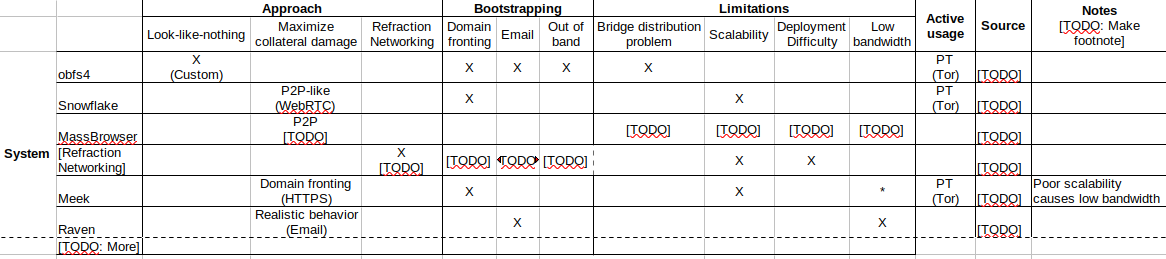
\includegraphics[width=\paperwidth]{tables/comparison-draft.png}}
\end{center}
\end{table}

We see that existing systems are limited by at least one of the following:
\begin{itemize}
  \item The bridge distribution problem [TODO: Xref]
  \item Scalability
  \item Deployment difficulty
  \item Low bandwidth
\end{itemize}

[TODO: More]

\section{Implementation}

TODO

\chapter{System evaluation}

TODO

\section{Performance}

TODO

\section{Bootstrapping availability}

TODO

\chapter{Conclusion}

TODO

\section{Future work}

TODO

\appendices  % Indicates that appendices follow.
% If there's only one, use \appendix instead.

\chapter{Sample appendix}
SAMPLE
\section{Sample section}
SAMPLE

\chapter{Second sample appendix}
SAMPLE


\bibliographystyle{plain}
\bibliography{lib/cites}

\end{document}

